\documentclass{article}
\usepackage{tikz}
\usepackage{amsmath,amssymb}
\usepackage{ifthen}
\usetikzlibrary{arrows,positioning,decorations.pathreplacing,shapes}
\usetikzlibrary{snakes} 
 
 
\begin{document}
 
\parindent=0em
 
\begin{center}
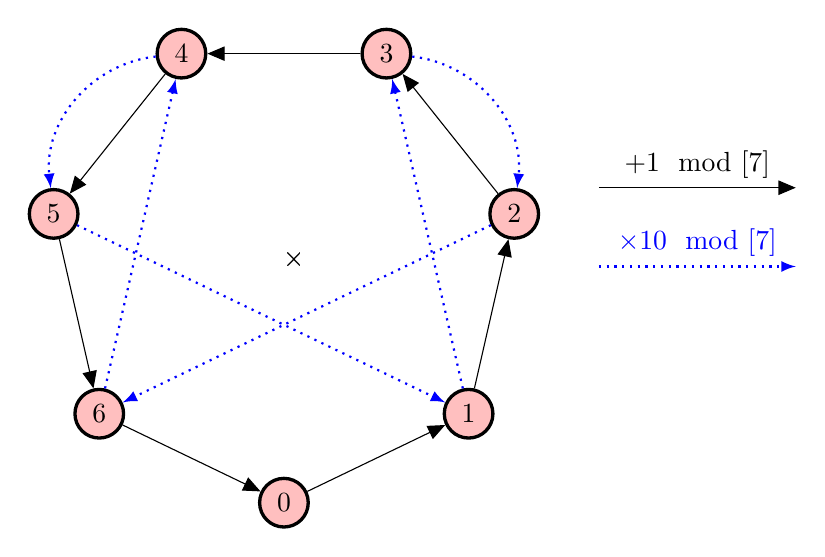
\begin{tikzpicture}
 
\def\n{7} %nombre de sommets du graphe
 
%%%%% Dessin des sommets %%%%%
\pgfmathtruncatemacro{\nmoinsun}{\n-1}
 
 
 
\foreach \x in {0,...,\nmoinsun}
\node[circle, very thick, draw=black, fill=red!25] (\x) at (270 + \x * 360/\n:3) {$\x$};
 
 
%%% Dessin des flèches noires %%%
 
\foreach \y in {0,...,\nmoinsun}
\pgfmathtruncatemacro{\z}{mod(\y +1, \n)} 
\draw[-triangle 45] (\y) to (\z);
 
 
%%%% Dessin des flèches bleues %%%%
 
 
\foreach \u in {1,...,\nmoinsun}
\pgfmathtruncatemacro{\v}{mod(\u * 10,\n)} 
\pgfmathtruncatemacro{\vplusun}{\v+1} 
\pgfmathtruncatemacro{\uplusun}{\u+1} 
\ifthenelse{\uplusun=\v}
					 {\draw[-latex, blue, thick, dotted] (\u) to[bend right=45] (\v);}
           {\ifthenelse{\vplusun=\u}
           				{\draw[-latex, blue, thick, dotted] (\u) to[bend left=45] (\v);}
           				{\draw[-latex, blue, thick, dotted] (\u) edge (\v);};};
 
 
 
 
\draw[-triangle 45] (4,1) -- node[above]{$+1 \mod [\n]$} (6.5,1) ;
\draw[-latex,  blue, thick, dotted] (4,0) -- node[above]{$\times 10 \mod [\n]$} (6.5,0) ;


Les flèches noires correpondent +1 modulo 7, les flèches bleues à ×10 modulo 7.
 
\end{tikzpicture}
\end{center}
 
\end{document}
